\documentclass[11pt,a4paper]{article}

\usepackage[utf8]{inputenc}
\usepackage[T1]{fontenc}
\usepackage[margin=2.5cm]{geometry}
\usepackage{graphicx}
\usepackage{booktabs}
\usepackage{amsmath}
\usepackage[hidelinks]{hyperref}
\usepackage{caption}
\usepackage{titlesec}
\usepackage{enumitem}
\usepackage{eurosym}
\usepackage{xcolor}
\usepackage{tikz}
\usetikzlibrary{positioning,arrows.meta}

% Deeper numbering, as in the reference report (2.4.1.1)
\setcounter{secnumdepth}{4}
\titleformat{\paragraph}[hang]{\normalfont\bfseries}{\theparagraph}{1em}{}
\setlist{nosep,leftmargin=1.4em}

% siunitx is available on Overleaf but not in the local check environment.
% These two macros give the same output with no package dependency, so the
% document compiles identically in both places. If you prefer real siunitx,
% add \usepackage{siunitx} and delete this block - the \SI calls are compatible.
\newcommand{\SI}[2]{#1\,#2}
\newcommand{\si}[1]{#1}
\newcommand{\percent}{\%}
\newcommand{\celsius}{\textdegree C}
\newcommand{\kilogram}{kg}\newcommand{\gram}{g}\newcommand{\hour}{h}
\newcommand{\per}{/}\newcommand{\metre}{m}\newcommand{\second}{s}
\newcommand{\milli}{m}\newcommand{\kilo}{k}
\newcommand{\SIrange}[3]{#1--#2\,#3}
\newcommand{\num}[1]{#1}

\title{\textbf{BladeLoop}\\[2mm]
\large Thermal Co-Processing of Decommissioned Wind Turbine Blades\\
\normalsize (Visualization of Process Engineering Applications)}

\author{%
Ritwika Sen \and Anirban Maji \and Akshat Daruka \and Sharan Murali \and
Anjani Lohith Kosana \and Hari Krishna Kondam}

\date{Digital Engineering Project, Summer Semester 2026\\
Otto-von-Guericke-Universit\"at Magdeburg\\[3mm]
\small Advisors: Dr.-Ing.\ David Broneske (Department of Computer Science)\\
\small Dr.-Ing.\ Nicole Vorhauer (Institute of Process Engineering)}

\begin{document}
\maketitle
\thispagestyle{empty}
\newpage

\tableofcontents
\newpage

\section{Introduction}

\subsection{Motivation}

Europe's first large generation of wind turbines is reaching the end of its life. Of the 290\,GW installed across Europe today, around 80\,GW will pass its theoretical operational lifetime by 2030, and the blades are the part that cannot simply be melted down and reused. WindEurope estimates annual blade waste will rise from roughly 20,000 tonnes in 2025 to about 55,000 tonnes by 2030, concentrated in the established markets of Germany and Spain \cite{windeurope}.

Until recently that material went to landfill. That route is closing. Germany has restricted the land-filling of composite waste, and the European wind industry adopted a self-imposed landfill ban that took effect on 1 January 2026 \cite{windeuropeban}. Disposing of a blade without carbon-fibre content costs on the order of 200 to 1,400 euros per tonne~\cite{envecon}. The waste has not gone away; it has become an obligation with a price attached.

That obligation is what creates the plant. Thermal co-processing --- pyrolysis in an oxygen-starved kiln turns a disposal liability into four recoverable streams: glass fibre, oil, gas and char. Plants of this kind are being built because the material has to go somewhere and landfill is no longer an option~\cite{noblade}.

Our starting point was the operators of those plants. A plant that must run, against orders from real buyers with real quality requirements, needs a way to decide how to run and that decision is not obvious from the chemistry alone. We set out to build something that shows it: take the order, set the plant, see what you made.

\subsection{Goals}

Regulation settles whether blades are recycled; it says nothing about how well. A plant built to satisfy a landfill ban still has to decide, every time an order arrives, how hard to run --- and that decision determines whether the recovered fibre is clean enough to sell into composites or only good enough to burn. The obligation is fixed. What comes out of it is not.

The aim was an interactive application, built for a plant operator rather than a chemist, that makes the consequences of a planning decision visible. It had to do four things.
\begin{enumerate}
  \item \textbf{Accept an order.} How much recovered material is wanted, how clean it has to be and work out settings for the plant that meet it.

  \item \textbf{Show the whole process.} From the wind farm to the separated outputs, as one continuous run, visualizing the entire process.

  \item \textbf{Make the trade-off visible.} Running the plant harder fills an order sooner but produces poorer material; running it gently costs time and blade stock. Neither is wrong. Which one is right depends on who is buying, and the application had to show that rather than assert it.

  \item \textbf{Report what actually happened.} Whether the run met what it was aiming at, what it consumed, and where every output ends up --- in a form the user can keep.
\end{enumerate}

All four exist for the same reason: so that an operator can see what a
decision will cost before committing to it, rather than after.

\subsection{Process Description}

A wind turbine blade is glass fibre held in a cured thermoset resin. The
choice is deliberate, it gives a structure that survives twenty years of fatigue loading and it is also what makes the blade difficult at end of
life. A thermoplastic can be melted and reformed. A thermoset cannot: the
resin is cross-linked, and heating it does not soften it back into something workable. The fibre inside is still valuable, but it cannot be separated mechanically without destroying it.

Thermal co-processing separates the two by decomposing the resin rather than melting it. The shredded blade material is held in a rotary kiln in the near-absence of oxygen, at a temperature the operator chooses: this model spans \SI{400}{\textdegree C} to \SI{700}{\textdegree C}, then ~\cite{bladegas} before the period. Without oxygen the resin cannot burn; starved of it, the polymer chains break apart instead, and the organic fraction leaves the solid as vapour. What remains in the drum is the glass fibre it was holding, together with whatever carbon the decomposition did not carry away.

Four streams come out of the process. The recovered \textbf{glass fibre} is the product the plant is run for. The vapour driven off is cooled, and the heavy fraction condenses as \textbf{pyrolysis oil} while the light fraction stays gaseous as \textbf{syngas}. The remainder is \textbf{carbon char} --- a solid carbon residue that decomposition left behind, separated from the fibre downstream by air classification~\cite{bladegas}, since char is light and fibre is not. A small fraction of the feed is lost entirely as fugitive dust and moisture.

\begin{figure}[htbp]
  \centering
  \resizebox{\textwidth}{!}{% Mass balance, high-grade design case.
% Every figure verified against ProcessModel.OutputSplit(). If the model
% changes, re-check these before trusting them.
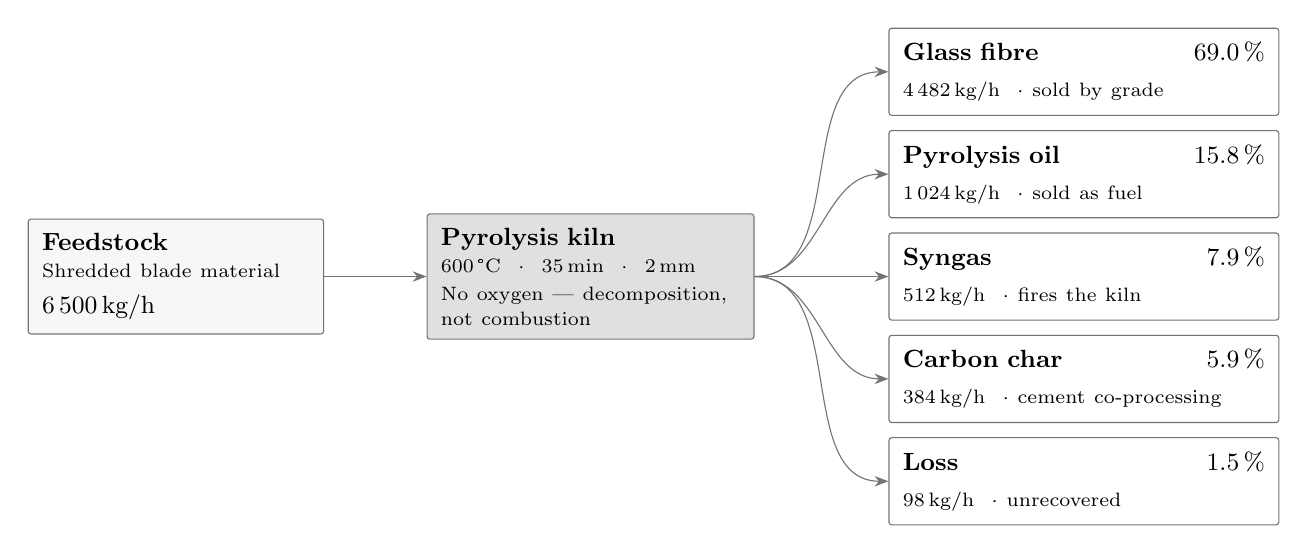
\begin{tikzpicture}[
  font=\small,
  box/.style={draw=black!55, rounded corners=1pt, align=left,
              inner sep=5pt, text width=46mm},
  src/.style={box, fill=black!3, text width=34mm},
  mid/.style={box, fill=black!12, text width=38mm},
  arr/.style={-{Stealth[length=5pt]}, draw=black!55}]

\node[src] (feed)
  {\textbf{Feedstock}\\[2pt]\scriptsize Shredded blade material\\[2pt]
   \small 6\,500\,kg/h};

\node[mid, right=13mm of feed] (kiln)
  {\textbf{Pyrolysis kiln}\\[2pt]
   \scriptsize 600\,\textdegree C \ $\cdot$ \ 35\,min \ $\cdot$ \ 2\,mm\\[2pt]
   \scriptsize No oxygen --- decomposition,\\[-2pt]\scriptsize not combustion};

\node[box, right=17mm of kiln, yshift= 26mm] (fib)  {\textbf{Glass fibre}\hfill 69.0\,\%\\[2pt]\scriptsize 4\,482\,kg/h \ $\cdot$\ sold by grade};
\node[box, right=17mm of kiln, yshift= 13mm] (oil)  {\textbf{Pyrolysis oil}\hfill 15.8\,\%\\[2pt]\scriptsize 1\,024\,kg/h \ $\cdot$\ sold as fuel};
\node[box, right=17mm of kiln]               (gas)  {\textbf{Syngas}\hfill 7.9\,\%\\[2pt]\scriptsize 512\,kg/h \ $\cdot$\ fires the kiln};
\node[box, right=17mm of kiln, yshift=-13mm] (char) {\textbf{Carbon char}\hfill 5.9\,\%\\[2pt]\scriptsize 384\,kg/h \ $\cdot$\ cement co-processing};
\node[box, right=17mm of kiln, yshift=-26mm] (loss) {\textbf{Loss}\hfill 1.5\,\%\\[2pt]\scriptsize 98\,kg/h \ $\cdot$\ unrecovered};

\draw[arr] (feed) -- (kiln);
\foreach \t in {fib,oil,gas,char,loss}
  \draw[arr] (kiln.east) to[out=0,in=180] (\t.west);

\end{tikzpicture}
}
  \caption{Output streams for the high-grade design case
           (\SI{600}{\textdegree C}, \SI{35}{min}, \SI{2}{mm} particle,
           \SI{6500}{kg/h} feed). Fibre purity is \SI{93.0}{\%} and tensile
           retention \SI{90.0}{\%}; the latter is a declared design constant
           rather than a literature-calibrated figure, discussed in
           Section~\ref{sec:assumptions}.}
  \label{fig:massbalance}
\end{figure}

Char is worth paying attention to, because it is the visible signal of an
incomplete process. Resin that breaks down fully leaves as oil and gas; resin that does not leaves as carbon on the fibre. A rising char fraction therefore means the kiln did not finish the job, and it is accompanied by exactly the effects one would expect --- less recovered fibre, and fibre that is less clean.

Four settings determine how completely that decomposition happens.
\textbf{Kiln temperature} sets how vigorously the resin cracks; too cool and it does not fully break down, too hot and the glass itself is damaged.
\textbf{Retention time} is how long material stays in the drum --- residence time in a continuous process, not a batch cycle. 
\textbf{Feed rate} sets throughput, and is bounded above by how quickly material can actually be heated through. 
\textbf{Particle size} governs heat transfer into each fragment, and in this model it is the most influential of the four: a coarse
particle does not reach temperature at its centre within the retention time available, so its interior is never properly processed regardless of how the kiln is set.

These settings are not independent, and they cannot all be optimised at once. Running hotter and faster moves more material per hour but degrades the fibre and drives up char. Running gently protects quality at the cost of throughput, which means more days and more blade stock consumed per tonne of product. There is no configuration that is best on every axis, which is why the application treats the choice as a trade-off rather than an optimisation with a single answer.

What decides which compromise is acceptable is the buyer. Recovered fibre is graded on two measures: \textbf{purity}, the fraction that is glass rather than residual carbon, and \textbf{tensile retention}, the proportion of original strength the fibre still carries. Three tiers follow, and each has a real market. Fibre at \SI{90}{\%} purity and \SI{85}{\%} tensile retention or better is clean and strong enough to return to structural composite parts. Below that, from \SI{78}{\%} and \SI{70}{\%}, it is no longer structural but sells as reinforcing filler for precast concrete~\cite{beauson2025}. Below that again it goes to cement co-processing, where the glass substitutes for raw silica in the kiln feed and any remaining organic content burns in place of coal~\cite{envecon}.

\begin{figure}[htbp]
  \centering
  \resizebox{0.95\textwidth}{!}{% Grade tiers and their buyers.
% Thresholds from OrderContext: High >= 90 purity / 85 tensile,
% Mid >= 78 / 70, Low below that. Keep in step with Section 1.3.
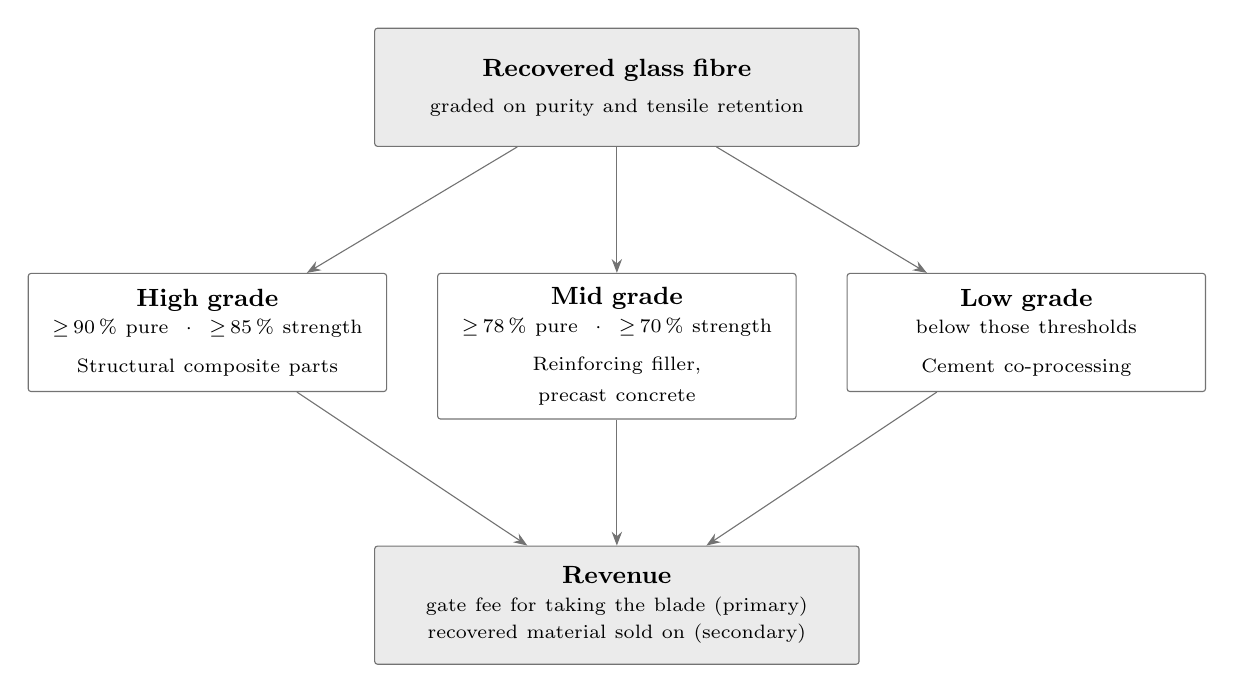
\begin{tikzpicture}[
  font=\small,
  box/.style={draw=black!55, rounded corners=1pt, align=center,
              inner sep=5pt, text width=42mm, minimum height=15mm},
  top/.style={box, fill=black!8, text width=58mm},
  arr/.style={-{Stealth[length=5pt]}, draw=black!55}]

\node[top] (src)
  {\textbf{Recovered glass fibre}\\[2pt]
   \scriptsize graded on purity and tensile retention};

\node[box, below=16mm of src, xshift=-52mm] (hi)
  {\textbf{High grade}\\[2pt]
   \scriptsize $\geq$\,90\,\% pure \ $\cdot$ \ $\geq$\,85\,\% strength\\[3pt]
   \scriptsize Structural composite parts};

\node[box, below=16mm of src] (mid)
  {\textbf{Mid grade}\\[2pt]
   \scriptsize $\geq$\,78\,\% pure \ $\cdot$ \ $\geq$\,70\,\% strength\\[3pt]
   \scriptsize Reinforcing filler, precast concrete};

\node[box, below=16mm of src, xshift=52mm] (lo)
  {\textbf{Low grade}\\[2pt]
   \scriptsize below those thresholds\\[3pt]
   \scriptsize Cement co-processing};

\node[top, below=16mm of mid] (rev)
  {\textbf{Revenue}\\[2pt]
   \scriptsize gate fee for taking the blade (primary)\\[-1pt]
   \scriptsize recovered material sold on (secondary)};

\foreach \t in {hi,mid,lo} \draw[arr] (src) -- (\t);
\foreach \f in {hi,mid,lo} \draw[arr] (\f) -- (rev);
\end{tikzpicture}
}
  \caption{Recovered fibre is graded, not passed or failed: each tier has a
           different buyer.}
  \label{fig:grades}
\end{figure}

This is the point on which the whole application turns. A run that misses the top tier has not failed; it has produced something a different customer will buy. An order specifies which tier it needs, and the settings that reach it follow from there.

\subsection{The Modelled Plant}

The application models a complete plant rather than a single apparatus, and the equipment it shows is the process design supplied by the chemical
engineering side of the team, built as 3D geometry and brought into the
application stage by stage. What follows is the material path through it.

\paragraph{Reception and size reduction.}
Blades arrive cut into sections, having been reduced on site to something a lorry can carry, and are fed onto a conveyor into a twin-shaft shredder. The two shafts counter-rotate, biting inward so that material is drawn down into the gap between them rather than thrown back out of the mouth. The shredder is where particle size is set --- the single most influential parameter in the process. Then its output is carried on a belt to the kiln feed.

\paragraph{Feed and airlock.}
Material cannot simply be tipped into the kiln, because the kiln's defining condition is the absence of oxygen. It enters instead through a feed tower fitted with a \textbf{rotary airlock valve}, which passes solids through while sealing against air. Below the valve a drop duct carries the charge into the kiln's feed housing. The airlock runs a repeating cycle --- accumulate, drop, purge --- so that at no point is there an open path from the room into the drum.

\paragraph{Pyrolysis.}
The \textbf{rotary kiln} is the centre of the plant: a slowly turning drum, modelled at \SI{1.5}{rpm}, heated externally by a burner ring and held under a nitrogen atmosphere. Rotation is what gives the process its retention time, tumbling material along the drum rather than letting it sit. The application divides the drum into the three zones the decomposition passes through --- \textbf{preheat}, \textbf{melting} and \textbf{char cracking} --- and offers a cutaway view, so the charge inside can be seen rather than inferred from the outside of a cylinder.

\paragraph{Discharge and solids handling.}
At the far end, the \textbf{discharge hood} performs the first separation
without any machinery at all: solids are too heavy to rise and fall out of the stream, while vapour climbs away. The solids leave down a \textbf{water-jacketed screw conveyor}, nitrogen-purged and cooling the
material from process temperature to around \SI{50}{\textdegree C}, because hot recovered fibre meeting air would oxidise and undo the work of the kiln. A second rotary airlock releases the cooled solids without admitting air behind them.

\paragraph{Air classification.}
The cooled solids are still a mixture of glass fibre and carbon char, and the two are separated by weight in a rising airstream: fibre is dense and drops out, char is light and is carried on. The fibre is collected and boxed; the char is drummed off separately.

\paragraph{The gas train.}
The vapour takes a longer path. A \textbf{gas-to-air heat exchanger} recovers some of its heat to preheat burner air. A \textbf{gas cyclone separator} spins out entrained char dust, which falls to its own bin --- a second, finer char stream distinct from the coarse char drummed off at the classifier. What remains is cooled in a \textbf{water-cooled condenser} to about \SI{45}{\textdegree C}, where the heavy fraction rains out as pyrolysis oil and is drawn off through a \textbf{gas--liquid separator}. The remaining non-condensable gas is drawn on by an \textbf{induced draft fan} and returned to the kiln burners~\cite{akesson,bladegas}, so part of the plant's own process heat is supplied by what it produces.

The five stages of the application follow this path in order --- wind farm, transport, shredding, kiln, separation --- so that the guided run traces the material rather than touring the equipment.

\subsection{Formulae and Calculations}
\label{sec:formulae}

The process model takes the four settings an operator controls and returns a closed mass balance, two quality measures and a grade. It is a surrogate model: fast enough to evaluate on every frame of an animation, which a full process simulation is not.

\subsubsection{Deviation from the design point}

Each setting has a design value, and what drives the model is not the setting itself but how far it sits from that value. Writing $T$ for kiln temperature, $t_r$ for retention time, $\dot{m}_f$ for feed rate and $d_p$ for particle size, with design values $\SI{600}{\textdegree C}$, $\SI{35}{min}$, $\SI{6500}{kg/h}$ and $\SI{2}{mm}$:

\begin{align}
  D_T   &= \min\!\left(\frac{|T - 600|}{150},\, 1\right) &
  D_{t}  &= \min\!\left(\frac{|t_r - 35|}{10},\, 1\right) \\[2pt]
  D_{\dot{m}} &= \min\!\left(\frac{|\dot{m}_f - 6500|}{2500},\, 1\right) &
  D_{d}  &= \min\!\left(\frac{\max(d_p - 2,\, 0)}{18},\, 1\right)
\end{align}

The particle term is deliberately one-sided. Material finer than the design point is not penalised --- a smaller fragment heats through more readily, not less, so only coarseness counts against the process.

These combine into a single weighted deviation:

\begin{equation}
  D = \min\bigl(0.30\,D_T + 0.22\,D_{t} + 0.16\,D_{\dot{m}} + 0.32\,D_{d},\; 1\bigr)
  \label{eq:D}
\end{equation}

Particle size carries the heaviest weight, slightly above temperature. Process efficiency is reported as $(1 - D) \times 100$, so the design case runs at \SI{100}{\%} by construction.

\subsubsection{Losses}

A fraction of the feed never becomes any product --- fugitive dust past the baghouse, moisture flash-off, and residue adhering to internal surfaces. It sits at a small baseline and climbs mainly with coarseness:

\begin{equation}
  f_{\text{loss}} = 0.015 + 0.085\,\bigl(0.75\,D_{d} + 0.25\,D\bigr),
  \qquad 0.015 \le f_{\text{loss}} \le 0.10
  \label{eq:loss}
\end{equation}

That is \SI{1.5}{\%} at the design case, rising to a capped \SI{10}{\%} at the worst reachable settings.

\subsubsection{Output split}

Losses are taken off the feed first; the remainder is shared between the four product streams. Their proportions at the design case follow the reference figures supplied by the process engineering side --- fibre 70, oil 16, syngas 8, char 6~\cite{akesson} and move with deviation:

\begin{align}
  g &= \operatorname{clamp}(70 - 26D - 12D_{d},\; 30,\; 72) \\
  o &= \operatorname{clamp}(16 - 6D,\; 4,\; 17) \\
  s &= \operatorname{clamp}(8 - 2D,\; 3,\; 9) \\
  c &= \operatorname{clamp}(6 + 24D + 12D_{d},\; 6,\; 42)
  \label{eq:props}
\end{align}

Fibre and char move in opposite directions and are the only two that respond to particle size directly: resin that fails to decompose leaves as carbon on the fibre rather than as oil or gas. Normalising over $\Sigma = g+o+s+c$ and applying the recovered fraction gives the mass flows:

\begin{equation}
  \dot{m}_i = \dot{m}_f \,(1 - f_{\text{loss}})\, \frac{i}{\Sigma},
  \qquad i \in \{g,\, o,\, s,\, c\}
  \label{eq:flows}
\end{equation}

The balance is closed by construction: the four product streams and the loss stream sum to the feed rate exactly, which the implementation asserts on every evaluation.

\subsubsection{Product quality}

Two measures describe the recovered fibre:

\begin{align}
  \text{purity} &= \operatorname{clamp}(93 - 17D - 19D_{d},\; 45,\; 93) \\
  \text{tensile retention} &= \operatorname{clamp}(90 - 36D_{d} - 11D_T - 9D_{t},\; 28,\; 90)
  \label{eq:quality}
\end{align}

Tensile retention does not depend on feed rate at all, and is dominated by particle size: its coefficient is more than three times that of temperature. This is the model's strongest statement that what damages recovered fibre is principally incomplete heating of coarse fragments, rather than the kiln being hot.

Purity here is a project definition rather than a published standard: the mass fraction of recovered material that is fibre, as against adhered char and resin residue. No standard expresses recovered fibre quality this way~\cite{pas101}, and the report uses the term only in that sense.

\subsubsection{Grade}

The two measures together place the output in one of three tiers, and both conditions must hold:

\begin{equation}
  \text{grade} =
  \begin{cases}
    \text{High} & \text{purity} \ge 90 \ \text{and}\ \text{tensile} \ge 85\\
    \text{Mid}  & \text{purity} \ge 78 \ \text{and}\ \text{tensile} \ge 70\\
    \text{Low}  & \text{otherwise}
  \end{cases}
  \label{eq:grade}
\end{equation}

\subsubsection{Campaign length}

Retention time is \emph{residence} time, not a batch cycle. The kiln is
continuous, so the material held inside it at any instant is
$\dot{m}_f \, t_r = \SI{6500}{kg/h} \times \SI{0.583}{h} = \SI{3792}{kg}$, and the time to fill an order follows from the hourly fibre rate rather than from $t_r$:

\begin{equation}
  t_{\text{campaign}} = \frac{m_{\text{order}}}{\dot{m}_g}
  = \frac{\SI{4800}{t}}{\SI{4.482}{t/h}} = \SI{1071}{h} \approx 44.6\ \text{days}
  \label{eq:campaign}
\end{equation}

This assumes continuous operation. At a more realistic \SI{85}{\%}
availability the same order takes 52.5 days.

\subsection{Assumptions and Their Basis}
\label{sec:assumptions}

The model in Section~\ref{sec:formulae} is a surrogate: a set of response curves fast enough to evaluate on every frame of an animation, fitted to behave the way the process behaves rather than derived from reaction kinetics. That choice buys interactivity and costs fidelity, and it is worth being explicit about where the cost falls.

\paragraph{Purity is our own definition.}
Of the two quality measures the application reports, only one can be checked against published work. Tensile retention is widely measured and widely reported. Purity, as we use it, the mass fraction of recovered material that is fibre rather than adhered char and resin residue --- has no published counterpart. The nearest comparable grading standard, PAS~101, governs container cullet glass and says nothing about composite-derived fibre~\cite{pas101}. So the purity half of every threshold in
Equation~\ref{eq:grade} is a project convention: internally consistent, usable for ranking one run against another, and not to be read as an industry figure.

\paragraph{Where the quality ceilings come from.}
The design case returns \SI{93}{\%} purity and \SI{90}{\%} tensile retention, and those ceilings were set deliberately rather than chosen for roundness. An earlier version of the model peaked at \SI{99}{\%} and \SI{100}{\%}, which amounts to claiming that thermal recovery does the fibre no harm at all. It does. Reviewing the literature in August 2026, the process engineering side of the team found recovered-fibre tensile retention spread across roughly \SIrange{72}{93}{\%}: ordinary single-step pyrolysis of real blade waste lands near \SI{72}{\%}~\cite{microwave}, a two-step route at \SI{425}{\textdegree C}
followed by \SI{475}{\textdegree C} oxidation reaches
\SI{76}{\%}~\cite{koh2021}, a two-temperature-step process improves on its single-step baseline by up to \SI{19}{\%}~\cite{twostep}, and only carefully optimised conditions approach \SI{93}{\%}~\cite{frpreview}. The ceilings were re-anchored to the top of that range, so the design case now represents best-in-class recovery rather than perfect recovery. The slopes were scaled by the same factor, so the shape of every response curve is unchanged --- only the anchor moved.

The same review found the grade thresholds themselves too generous. They had been set at \SI{95}{\%} purity and \SI{95}{\%} tensile retention for high grade, a bar above almost every published result. They were lowered to \SI{90}{\%} and \SI{85}{\%}, which is where the thresholds in Equation~\ref{eq:grade} come from.

\paragraph{The process we depict and the numbers we quote.}
This is the assumption we are least comfortable with, and it is better stated than discovered. The figures above come from specialised routes --- microwave pyrolysis, potassium-hydroxide-assisted two-step treatment, molten-salt-assisted recovery~\cite{moltensalt}. What the application depicts is a conventional rotary kiln followed by air classification, and that is the route for which the more pessimistic figures in the literature apply: where recovered fibre is cleaned of char oxidatively, tensile retention measured against virgin fibre falls a great deal further, to somewhere between a third and a half of original
strength~\cite{feih2011,feih2015,conditioning2014}. The damage there is done largely by the cleaning step rather than by the heating.

So the model is anchored to what the best recovery processes achieve, while the plant on screen is a conventional one. A stricter model would either depict a different plant or report lower numbers. We have kept the anchoring and named the gap, because the application's purpose is to show how a planning decision moves the outputs and the direction and relative magnitude of every response survive the re-anchoring, even where the absolute values sit optimistically.

\paragraph{Gas-only firing is close to break-even.}
Stage~4 of the guided run states that the recovered gas fires the kiln while the oil is sold on. Pyrolysis oil from blade waste carries
\SIrange{34}{36}{MJ/kg}~\cite{akesson}, which makes selling it the right
decision; the gas fraction is dominated by carbon dioxide and carbon monoxide and carries far less. Published gas calorific values for blade pyrolysis convert to roughly \SIrange{15}{20}{MJ/kg} on a mass
basis~\cite{bladegas,torres}. Against the kiln's estimated heat demand, that puts gas-only firing between \num{0.73} and \num{1.13} times what the kiln needs, depending on which end of the published range is taken and which grade is being run. The claim is therefore plausible rather than proven, and the low grade is the most marginal case. This reflects real uncertainty in the published figures for this material, not a flaw in the plant design.

\paragraph{Campaign length assumes continuous operation.}
Equation~\ref{eq:campaign} divides an order by the hourly fibre rate and reports the result directly, which assumes the plant runs without interruption. Real plants do not. At a more representative \SI{85}{\%} availability every campaign length in the application is roughly a sixth longer --- the \num{4800}-tonne order shown becomes \num{52.5} days rather than \num{44.6}. The application reports the continuous figure because it is the one that follows from the settings the user chose, and adding an availability factor would obscure the relationship the screen exists to show.

\paragraph{The feedstock is treated as one material.}
A single composition enters the kiln, and it does not vary. Real decommissioned blades do: resin systems differ between manufacturers and between generations of the same manufacturer, the material has spent two decades weathering, and a blade section arrives with balsa or foam core, bonded-in steel root fixings, paint and leading-edge protection still attached. Any of those changes what the kiln produces, and a plant taking mixed blade stock would see run-to-run variation that this model has no way to express. The four settings are the only thing that
moves the outputs, which is a considerable simplification of what determines them.

\paragraph{The four settings are treated as independent.}
The application lets each of the four be set without reference to the others, and a real plant could not. Feed rate and retention time are coupled through the drum: for a kiln of fixed volume and inclination, pushing more material through per hour shortens the time any of it spends inside, so the highest feed rate and the longest retention time cannot be selected together. The model permits it. The simplification is deliberate as the application exists to show what each
lever does, and a user who cannot move one lever without the others moving underneath them cannot see that --- but it means some of the reachable settings describe a plant that could not be built to that specification.

\paragraph{Feed rate and particle size are bounded by the design, not by
physics.}
The ranges the sliders offer --- \SIrange{400}{700}{\textdegree C},
\SIrange{25}{45}{min}, \SIrange{4000}{9000}{kg/h}, \SIrange{0.5}{20}{mm} --- describe the plant as designed rather than the limits
of the chemistry. Settings outside them are not represented, and the model should not be read as predicting what would happen there.

\section{User Documentation}

\subsection{Minimum Software Requirements}

BladeLoop is a standalone Windows application. It needs Windows~10 or later on a 64-bit machine, a graphics adapter supporting DirectX~11, and roughly \SI{2}{GB} of free disk space for the unpacked build. No runtime, framework or supporting software has to be present: the build ships with everything it needs.

A mouse with a scroll wheel is a requirement rather than a preference. Explore mode orbits the camera on left-drag and zooms on scroll, and a trackpad without scroll gestures leaves the zoom unreachable. Sound is optional, the narration is subtitled throughout but the run is written to be heard, and the subtitles carry the words rather than the emphasis.

\subsection{Installation and Configuration}

There is no installer. The application is distributed as a folder containing \texttt{BladeLoop.exe} and its data directory; unpack it anywhere and run the executable. The two must stay together --- moving the executable out of its folder leaves it unable to find its data. Because the build is unsigned, Windows may show a SmartScreen warning the first time it runs, which is cleared through
\emph{More info} $\rightarrow$ \emph{Run anyway}.

Nothing needs to be configured. The application stores no settings, requires no account and writes nothing to disk except the run report, and then only when the user asks for it. Uninstalling is deleting the folder.

It launches fullscreen at the desktop resolution. \textsc{alt}+\textsc{enter} switches to a window, which can then be resized freely; the interface re-flows to whatever it is given. The guided run is composed for a landscape frame, though the camera shots assume a wide viewport, and in a narrow window the order panel takes a share of the width that leaves little for the plant.

\subsection{Scene Description}

The application is built from three kinds of scene. The \textbf{home page} and \textbf{Custom Order} screens are interface: they collect an order and set the plant. The \textbf{How It Works} screen explains the process without running anything. The \textbf{guided run} is five scenes played in sequence, each one stage of the plant, cut together so the material is followed from the wind farm to the separated products rather than the equipment being toured.

\begin{table}[htbp]
  \centering
  \caption{Stages of the guided run.}
  \label{tab:stages}
  \begin{tabular}{llr}
    \toprule
    Stage & Subject & Duration \\
    \midrule
    1 & Wind farm and decommissioning & \SI{23.8}{s} \\
    -- & Transport (pass-through)      & \SI{9.6}{s} \\
    2 & Shredding                      & \SI{30.4}{s} \\
    3 & Rotary kiln                    & \SI{33.6}{s} \\
    4 & Separation and by-products     & \SI{46.7}{s} \\
    \midrule
    & Total & \SI{144.1}{s} \\
    \bottomrule
  \end{tabular}
\end{table}

The run is continuous: stages hand off to one another without returning to a menu, and the transport segment between the wind farm and the shredder is a pass-through rather than a stage in its own right. Total running time is a little over two minutes.

\subsection{Process Scene Details --- Navigation and User Interface}

\subsubsection{Placing an order}

Everything the plant does follows from an order, and the home page offers two ways to place one: run a worked example, or build an order from scratch.

\paragraph{Worked examples.}
Three preset orders sit on the home page, one per grade. They are not three arbitrary demonstrations --- each is the same decommissioned wind farm sold to a different customer, which is what makes them worth comparing.

\begin{table}[htbp]
  \centering
  \caption{The three worked examples. All three consume the same feedstock ---
           approximately \SI{6990}{t} of blade material, \num{619} blades from
           \num{206} turbines --- and differ only in who is buying.}
  \label{tab:presets}
  \begin{tabular}{llrrrrr}
    \toprule
    Buyer & Grade & Order & Temp. & Retention & Feed & Particle \\
    \midrule
    Composite manufacturer & High & \SI{4800}{t} & \SI{600}{\textdegree C} & \SI{35}{min} & \SI{6500}{kg/h} & \SI{2}{mm} \\
    Precast concrete producer & Mid & \SI{4100}{t} & \SI{580}{\textdegree C} & \SI{35}{min} & \SI{8000}{kg/h} & \SI{8}{mm} \\
    Cement works & Low & \SI{3250}{t} & \SI{550}{\textdegree C} & \SI{35}{min} & \SI{8800}{kg/h} & \SI{16}{mm} \\
    \bottomrule
  \end{tabular}
\end{table}

The tonnages differ because the grades differ: coarser settings recover less fibre per tonne of blade, so the same farm yields less product when it is run for cement co-processing than when it is run for structural reuse. Selecting a card places the order and starts the run immediately.

\paragraph{Custom Order.}
The Custom Order screen builds an order in four steps --- \textsc{what you know}, \textsc{your numbers}, \textsc{what matters to you}, \textsc{your plan} --- with one question open at a time and completed steps collapsed to a single line. Steps can be reopened; nothing is committed until the last one.

The first step asks what the user already has, because different users arrive knowing different things. \emph{I know my buyer} suits someone selling to a specific customer and works backwards from the grade that customer needs. \emph{I have material} suits a yard full of blades and no order yet. \emph{I have a constraint} suits an operator whose shredder only goes so fine, and works forwards from the equipment to what it can produce. All three converge on the same place: a plan --- a set of four plant settings --- that the run will then execute.

The plans offered at the last step are drawn from a frontier of non-dominated options: settings that no other setting beats on both the grade reached and the time taken. A slider moves along that frontier, trading days against quality, and the consequences of each position are shown as it moves. Any plan can also be edited directly, at which point it leaves the frontier and becomes whatever the user made it.

\subsubsection{Watching the run}

\paragraph{The order panel.}
A panel occupies the right of the frame throughout the run and is the part of the screen that is not a video. It tracks the four settings and the five output streams, and it fills in progressively: each setting appears as the run reaches the equipment that decides it, so particle size arrives at the shredder and temperature at the kiln rather than all four being present from the start. Alongside each value the panel shows the design case as a reference mark, so a setting can be read as a distance from the design point rather than as a bare number.

\paragraph{Explore mode.}
Pressing \textsc{space} or \textsc{p} at any point pauses the run and hands the camera over. The view can then be orbited by dragging with the left mouse button and zoomed with the scroll wheel, pivoted on whatever the shot was framing when it was paused. Pressing the same key resumes, and the camera returns to the composed shot.

Pausing stops the entire scene, not just the camera: the timeline, the narration and every script-driven animation --- kiln rotation, conveyors, the airlock cycle --- hold their positions, so the paused frame is a frozen plant rather than a still plant with machinery running in it. Some equipment can also be opened while paused, where a cutaway view exists for it.

\paragraph{Subtitles and navigation.}
Narration is subtitled throughout, at the foot of the frame. Three controls sit over the run: \textsc{menu} at the top left returns to the home page, \textsc{skip intro} at the top right jumps past the opening stages to the plant itself, and \textsc{previous} and \textsc{next stage} step between stages. The stage controls grey out where there is nowhere to go --- there is nothing before the wind farm and nothing after separation --- rather than disappearing, so the frame does not reflow as the run progresses. Pressing \textsc{escape} leaves the
run and returns to the home page.

\subsubsection{Reading the outcome}

When the last stage ends, the order panel expands from its column to fill the frame and becomes the run report. It opens with the verdict --- \emph{order filled} or \emph{target missed} --- and then sets out, in five parts, what the run did:

\begin{itemize}
  \item \textbf{The order}: the buyer, the grade requested and the tonnage.
  \item \textbf{How the plant was set}: the four settings, each shown against
        its design value.
  \item \textbf{What the plant made}: the five output streams as shares and as
        mass flows, each with the design-case share marked for comparison.
  \item \textbf{Fibre quality}: purity, tensile retention, the grade reached and
        the process efficiency.
  \item \textbf{What the run costs}: blade material consumed, blades, turbines
        and campaign length.
\end{itemize}

The report is the answer to the question the application asks on the home page, and it is deliberately not a score. A run that misses its target has still produced something, and the report says who buys it. The whole report can be saved as a single self-contained HTML file, which opens in any browser and needs nothing from the application to read.

\section{Developer Documentation}

\subsection{Tool Suite}

The application is built in \textbf{Unity 6} (6000.4.7f1) against the Universal Render Pipeline. Four Unity packages carry most of the weight: \textbf{Cinemachine~3} for the camera work, \textbf{Timeline} for the choreography of each stage, the \textbf{Input System} for keyboard and mouse handling, and \textbf{TextMesh~Pro} for all typography. Everything is written in C\#; there is no visual scripting in the shipped code.

Geometry is modelled in \textbf{Blender} and exported to FBX. The source
\texttt{.blend} files are kept in the repository alongside the exports, so a piece of equipment can be revised without reconstructing it from the imported mesh. Narration was recorded and edited externally and enters the project as audio clips placed on Timeline tracks.

The chemical engineering side of the team worked in \textbf{DWSIM} for process modelling and \textbf{OpenLCA} for impact assessment. Neither runs inside the application, their role was to establish the reference figures that Section~\ref{sec:formulae} is fitted to, and those figures enter the codebase as constants rather than as a live link.

Source control is \textbf{Git}, hosted on GitHub, with Git~LFS for binary
assets. Work was organised as one branch per feature with review before merge, which matters more than usual here for the reason set out in
Section~\ref{sec:scenemerge}.

\subsection{Class Hierarchy}

There are around seventy C\# files and roughly \num{15000} lines. They fall into six groups, and the division that matters most is the first one: the process model knows nothing about Unity.

\begin{table}[htbp]
  \centering
  \caption{The six layers, and what each is allowed to know about.}
  \label{tab:layers}
  \begin{tabular}{p{3.4cm}p{4.2cm}p{6.2cm}}
    \toprule
    Layer & Principal classes & Responsibility \\
    \midrule
    Process model &
      \texttt{ProcessModel}, \texttt{PlantModel}, \texttt{OrderSolver} &
      The equations of Section~\ref{sec:formulae} and the search for settings
      that meet an order. Plain C\#, no Unity types, independently testable. \\
    \addlinespace
    Shared state &
      \texttt{OrderContext} &
      The current order, the current plan and the last run's results. Static,
      so it survives scene loads without a carrier object. \\
    \addlinespace
    Screens &
      \texttt{MainMenuController}, \texttt{OrderDashboardController},
      \texttt{HowItWorksController} &
      The three interface scenes. Each builds its own layout in code at
      runtime. \\
    \addlinespace
    Run control &
      \texttt{TourRunner}, \texttt{TourSceneSequencer},
      \texttt{StoryModeController}, \texttt{TourControls},
      \texttt{SubtitleTrack} &
      Sequencing the five stages, pausing, subtitles and the controls
      overlaid on the run. \\
    \addlinespace
    Order-driven binders &
      \texttt{KilnOrderBinding}, \texttt{Stage4OrderBinding},
      \texttt{ShredOutputSizer}, \texttt{KilnShellGrade},
      \texttt{SeparationController} &
      The bridge: read the order, change what the scene shows. Discussed in
      Section~\ref{sec:binders}. \\
    \addlinespace
    Scene animation &
      \texttt{KilnRotator}, \texttt{ConveyorBeltScroller},
      \texttt{AirlockDoorCycle}, \texttt{WorkerPatrol} and some thirty others &
      Small single-purpose behaviours that move one thing. Deliberately
      unaware of the order. \\
    \addlinespace
    Output &
      \texttt{OrderPanel}, \texttt{OutcomeReport},
      \texttt{OutcomeReportPanel} &
      The live panel during the run and the report at the end. \\
    \bottomrule
  \end{tabular}
\end{table}

Two decisions in that table are worth defending.

\textbf{The process model has no Unity dependency.} \texttt{ProcessModel} is a plain class with float properties, and it can be evaluated without a scene, a camera or a running game. That is what made it possible to check the constants against the reference figures by running the model directly, and to verify that the mass balance closes on every evaluation rather than hoping it does.

\textbf{\texttt{OrderContext} is static rather than a singleton
\texttt{MonoBehaviour}.} The conventional Unity pattern for cross-scene state is an object marked \texttt{DontDestroyOnLoad}, which requires that some scene create it, that no scene create it twice, and that every consumer find it. A static class needs none of that: the home page writes to it, five stage scenes read from it, and nothing has to be wired in the inspector. The cost is that it cannot be inspected while the game runs, which is a fair trade for state this small.

\subsection{Implementation Specifics}

\subsubsection{Scene files cannot be merged}
\label{sec:scenemerge}

A Unity scene is a YAML file of serialised objects keyed by generated file IDs. Two developers editing the same scene produce two files that Git will cheerfully merge line by line into something Unity cannot open --- and the failure is not a conflict marker in a source file but a corrupted scene, sometimes one that opens and is subtly wrong rather than one that refuses to load.

This is a well-known Unity problem, and the usual answers did not fit a project of this size and duration. So the rule was simply that \textbf{every scene has one owner}, and only that person edits it. What made the rule survivable was building interface in code rather than in the editor: \texttt{MainMenuController}, \texttt{OrderDashboardController} and \texttt{OrderPanel} construct their entire layouts at runtime, so the scene asset holds almost nothing and the layout lives in a C\# file that merges normally. Several components bootstrap themselves through \texttt{[RuntimeInitializeOnLoadMethod]} and are therefore present in no
scene at all.

The consequence for anyone extending the project is that adding a button is a code change, not an editor change, and looking for the interface in the scene hierarchy will not find it.

\subsubsection{Order-driven visuals}
\label{sec:binders}

Nothing in the guided run is prerecorded. The same five scenes play for every order, and what differs is what they show --- which is arranged through a consistent pattern.

Each stage carries a \emph{binder}: a component that reads
\texttt{OrderContext} once, computes what the scene should look like, and writes that into the scene's animation components. \texttt{ShredOutputSizer} sets the size and spacing of the fragments on the belt from the particle size. \texttt{KilnOrderBinding} and \texttt{TemperatureRampAnimator} drive the kiln's
emissive glow from the temperature, across the hundred and thirteen renderers that make up the drum, its burner ring and its housing.
\texttt{Stage4OrderBinding} sets the emission rates of the oil, syngas and char particle streams from the computed output split, and rewrites the temperature labels on the equipment so they agree with the run.

The point of the pattern is that the thirty-odd small animation behaviours know nothing about orders. \texttt{KilnRotator} turns a drum; it does not know why. That keeps the parts that had to be edited by several people over several months simple, and concentrates order-awareness in six binder classes that one person maintained.

\subsubsection{Problems encountered}

Five faults are worth recording, because each was found late, none produced an error message, and the reason each was hard to see is more instructive than the fix.

\paragraph{Choreography written in absolute seconds.}
This one recurred five separate times, in five unrelated places, and is the single most expensive mistake in the project. Animation phases were written as absolute times --- open the door at \SI{3}{s}, start the purge at \SI{4.6}{s} --- which is correct until the sequence they belong to is retimed. When Stage~4 was shortened from \SI{86}{s} to \SI{46.7}{s}, everything keyed to absolute seconds silently desynchronised: doors opened after the camera had moved on, a cutaway revealed an interior that was no longer there. Nothing threw an exception; the scene simply stopped telling the truth.

The fix, applied everywhere it applied, is to express every phase as a
\emph{fraction} of the sequence it belongs to, so retiming carries the
choreography with it. In \texttt{AirlockDoorCycle} the three phases became $3/6$, $4/6$ and $4.6/6$ of the cycle length --- written as exact divisions rather than as decimals, because rounding $4/6$ to \num{0.6667} moved two boundary frames, which a sweep of twelve hundred samples caught and inspection would not have.

\paragraph{Two components writing the same property.}
The kiln's shell colour was driven by \texttt{TemperatureRampAnimator} at
default execution order, and by \texttt{KilnOrderBinding} at order~60. Unity runs them in that order, so the second silently overwrote the first every frame and the shell stopped responding to temperature. Nothing was wrong with either class in isolation, which is why it survived review: the bug existed only in the relationship between them. It was found by a team member watching the kiln in play mode and noticing it did not change --- a test that would never have caught
it, because the value was correct right up until it was overwritten. The fix was to make the ordering explicit through \texttt{[DefaultExecutionOrder]} across the whole family of components rather than to let it fall out of defaults.

\paragraph{\texttt{GameObject.Find} does not see inactive objects.}
Several particle systems in Stage~4 begin disabled and are enabled when the run reaches them. Looking them up with \texttt{GameObject.Find} returns \texttt{null}, and a null check that quietly skips the missing object turns the whole feature into a no-op that logs nothing. The stream appeared to be wired and did nothing. Every lookup of this kind now goes through \texttt{FindObjectsByType} with \texttt{FindObjectsInactive.Include}.

\paragraph{Pausing a Timeline by setting its speed to zero stops the audio.}
Explore mode pauses the run, and the obvious implementation --- set the playable graph's speed to zero --- worked for everything visible and broke the narration. Audio cannot play at zero rate, so Timeline stopped the voice-over source rather than pausing it, and never rescheduled it on resume: the narration went silent for the rest of the stage. \texttt{PlayableDirector.Pause()} and \texttt{Resume()} are the supported path and keep audio scheduling intact. Pausing correctly also turned out to need \texttt{Time.timeScale} and the Cinemachine brain handled separately, because the script-driven animations and
the camera run on clocks the director does not own.

\paragraph{\texttt{Renderer.material} and \texttt{Renderer.sharedMaterial}.}
Reading \texttt{renderer.material} instantiates a per-object copy;
\texttt{sharedMaterial} returns the project asset itself. Writing to the latter at runtime edits the asset on disk --- in the editor the change persists after play mode ends, so a debugging session can permanently alter the project's materials without any indication that it has. The heat ramp writes to \texttt{material} for exactly this reason, and the distinction is noted at the line where it matters.

\paragraph{What these have in common.}
None of the five produced an error. Every one of them was a component doing precisely what it was told, in a context where that was the wrong thing which is the characteristic failure mode of a system assembled from small independent behaviours. The defence that worked was not more testing but fewer implicit relationships: explicit execution order, choreography expressed relative to its container, and lookups that state what they expect to find.
\section{Conclusion}

\subsection{Results}
% What was built, and the argument it makes: there is no single correct
% setting, and the buyer decides the quality bar.
\textit{[prose]}

\subsection{Why Recycled Fibre Is Bought At All}
% The economics answer to the professor's question. Short version:
% on price and performance alone it loses; the case is on the disposal side.
%  - virgin E-glass ~$1.30/kg \cite{techecon}
%  - recovered fibre must sell at ~80% of virgin to break even
%  - EU landfill ban from 1 Jan 2026; disposal EUR 200-1400/t
%  - the gate fee is the primary revenue; recovered streams are secondary
%  - embodied energy: ~2.0-2.6 MJ/kg of fibre here vs 20-30 MJ/kg virgin
\textit{[prose]}

\subsection{Outlook}
\textit{[prose]}


\bibliographystyle{unsrt}
\bibliography{refs}

\end{document}
